La gráfica de una esfera se pueden representar del siguiente modo:

\begin{figure}[H]
  \centering
  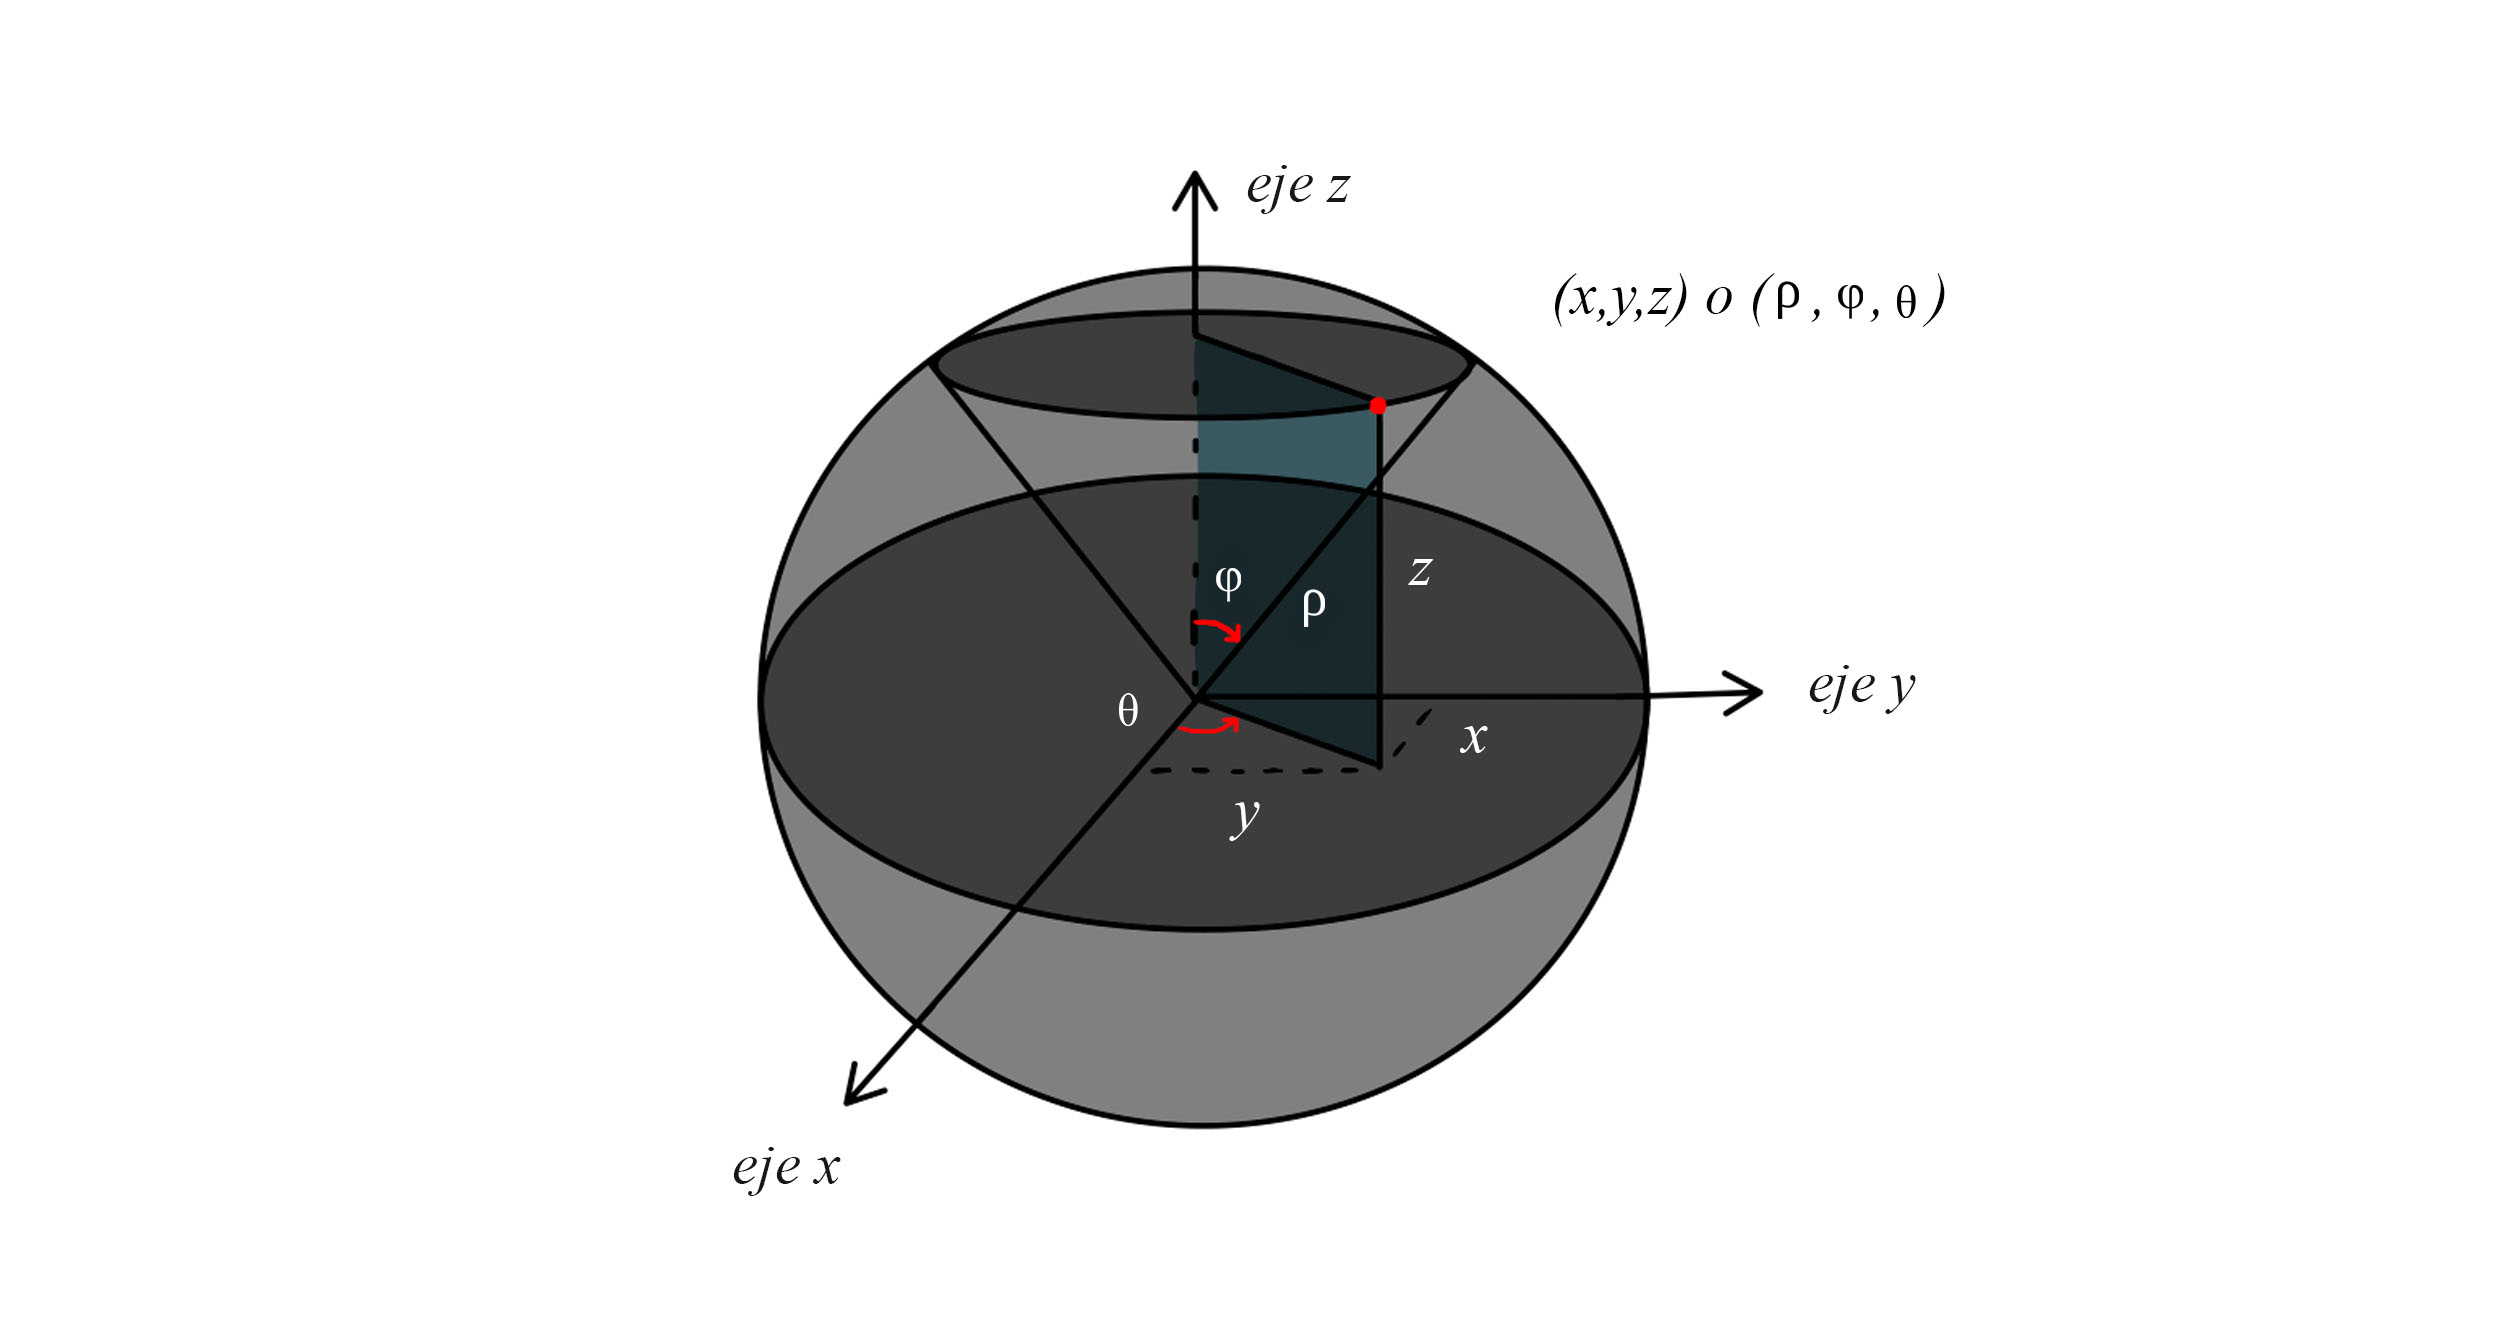
\includegraphics[width=11.17cm, height=5.97cm]{img/graph/sfera.jpg}
  \caption{Una esfera.}
\end{figure}

% --TODO: Incluir gráfica genérica, la que tú quieras [img/graph/grafica_generica.jpg]

Usando ejemplos más concretos, se pueden graficar los siguientes puntos y su representación es la siguiente:

\vspace{4mm}
Gráfica de la coordenada ${\left( 6,\frac{\pi}{3},\frac{\pi}{6} \right)}$ donde: ${\theta = \frac{\pi}{3} = 60^{\circ} }$ y ${ \varphi = \frac{\pi}{6} = 30^{\circ}}$.
\begin{figure}[H]
  \centering
  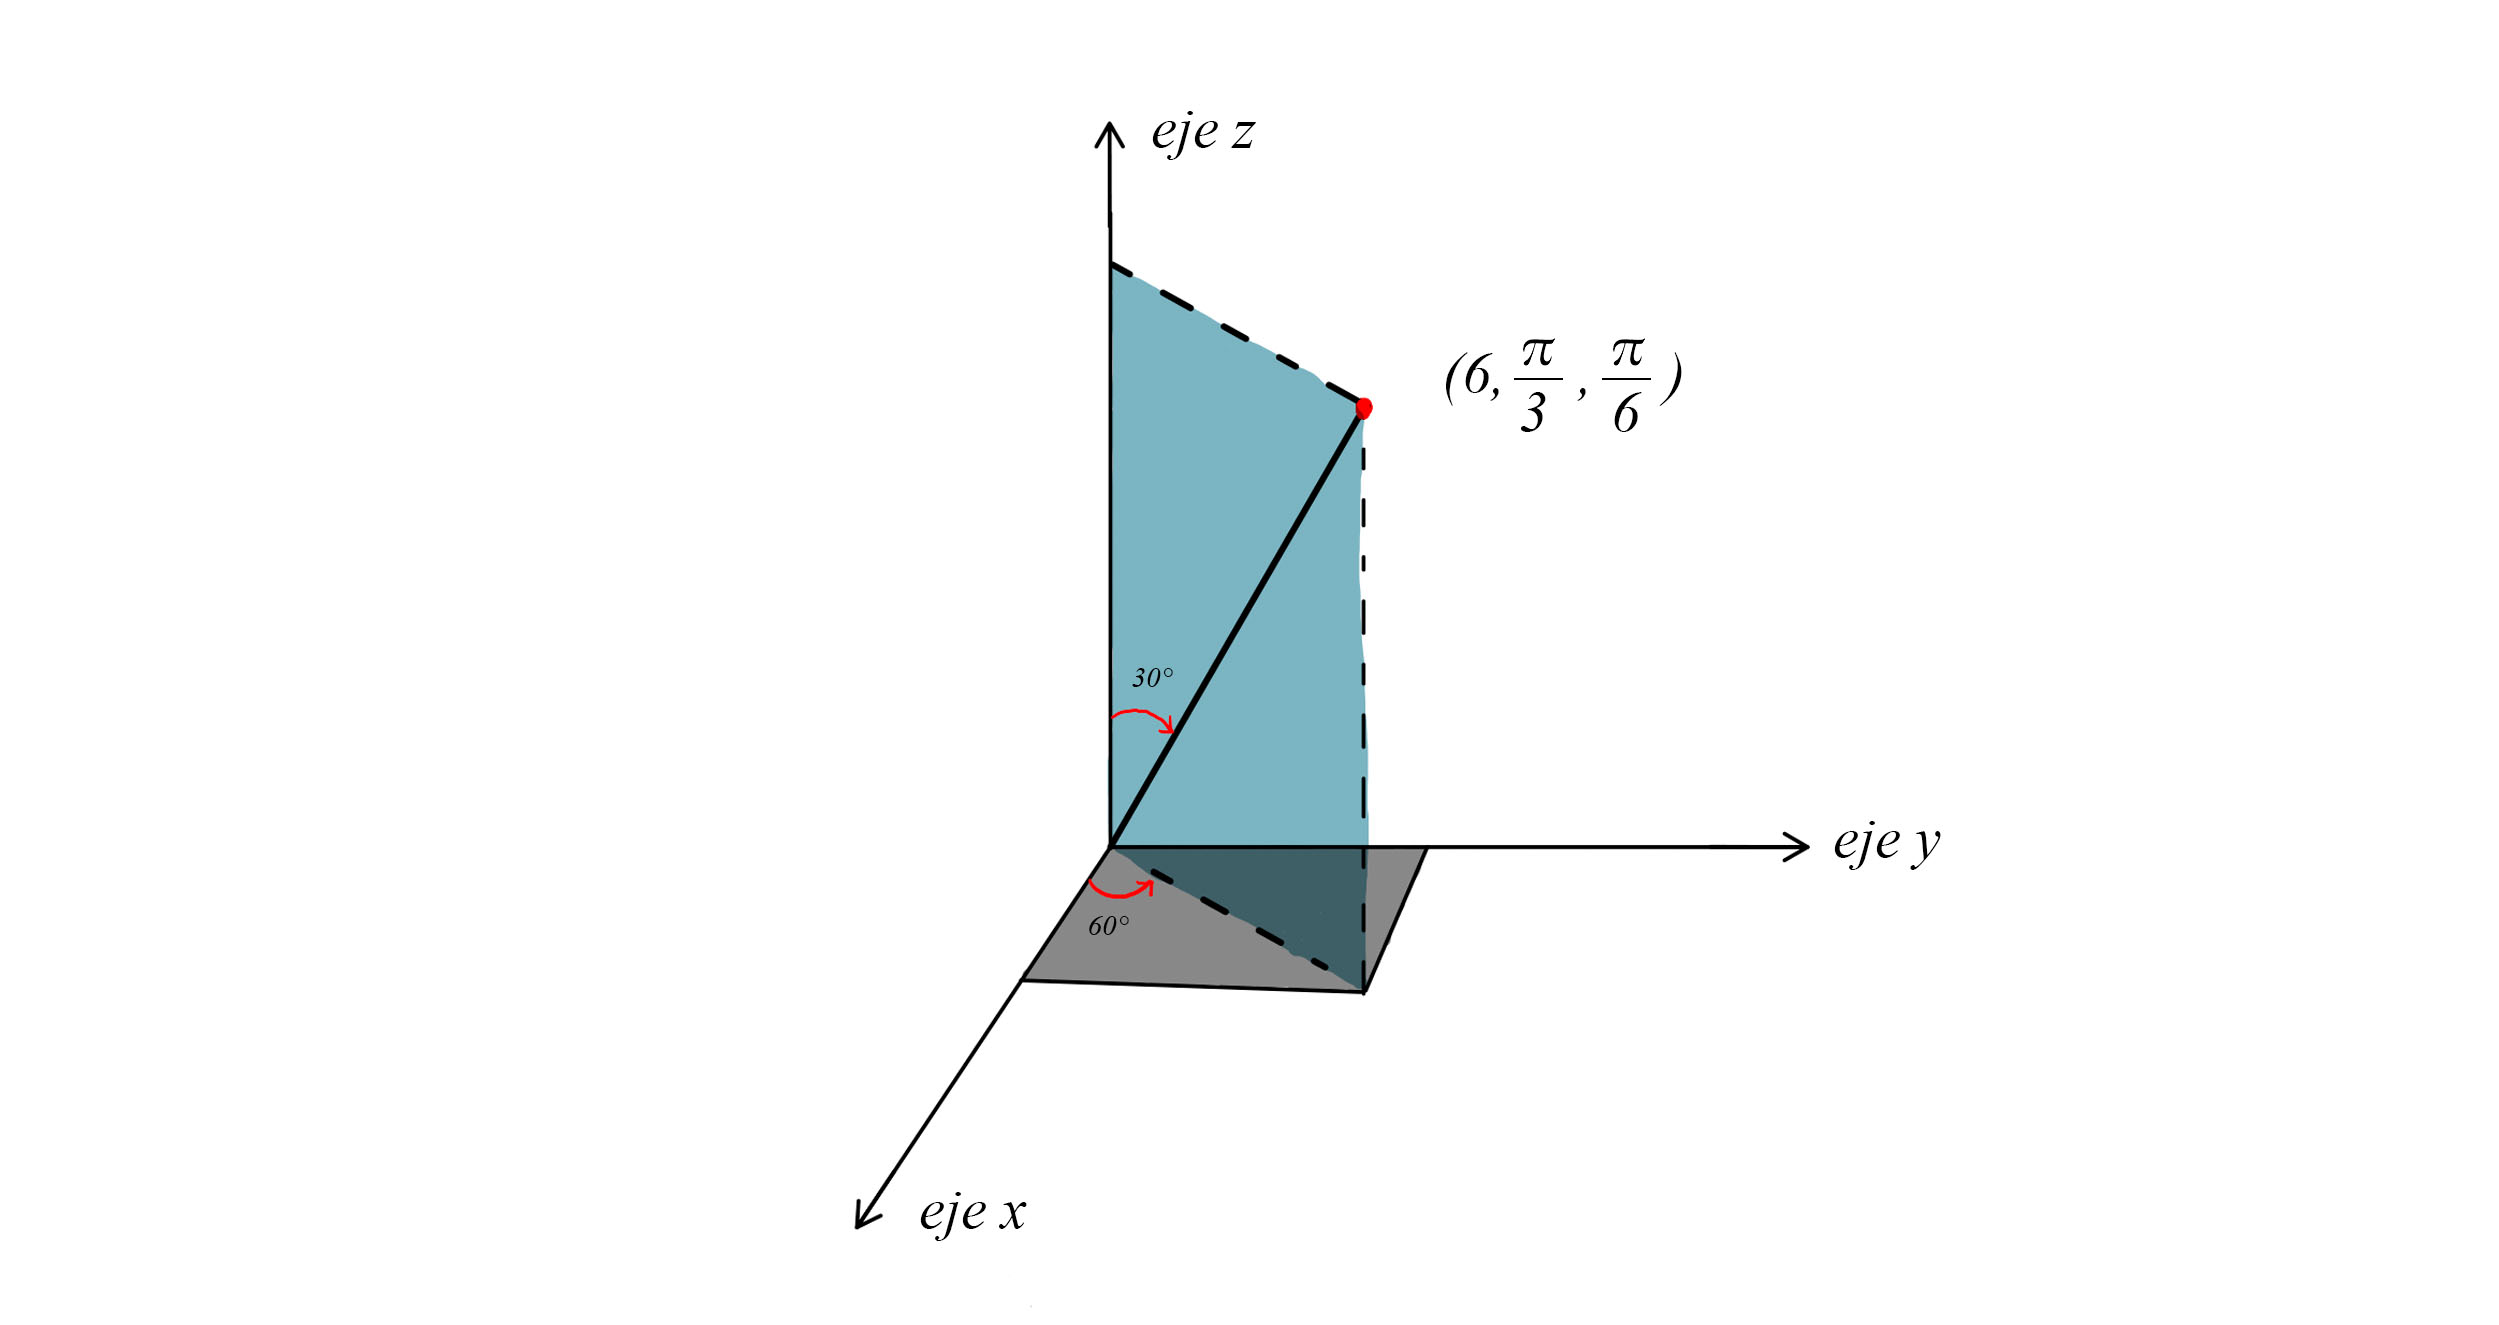
\includegraphics[width=11.17cm, height=5.97cm]{img/graph/grafica_1.jpg}
  \caption{Coordenada ${\left( 6,\frac{\pi}{3},\frac{\pi}{6} \right)}$.}
\end{figure}

\vspace{4mm}
Gráfica de la coordenada esférica ${\left( 3, 0,\frac{\pi}{3} \right)}$ donde: ${ \varphi = \frac{\pi}{3} = 60^{\circ} }$.
\begin{figure}[H]
  \centering
  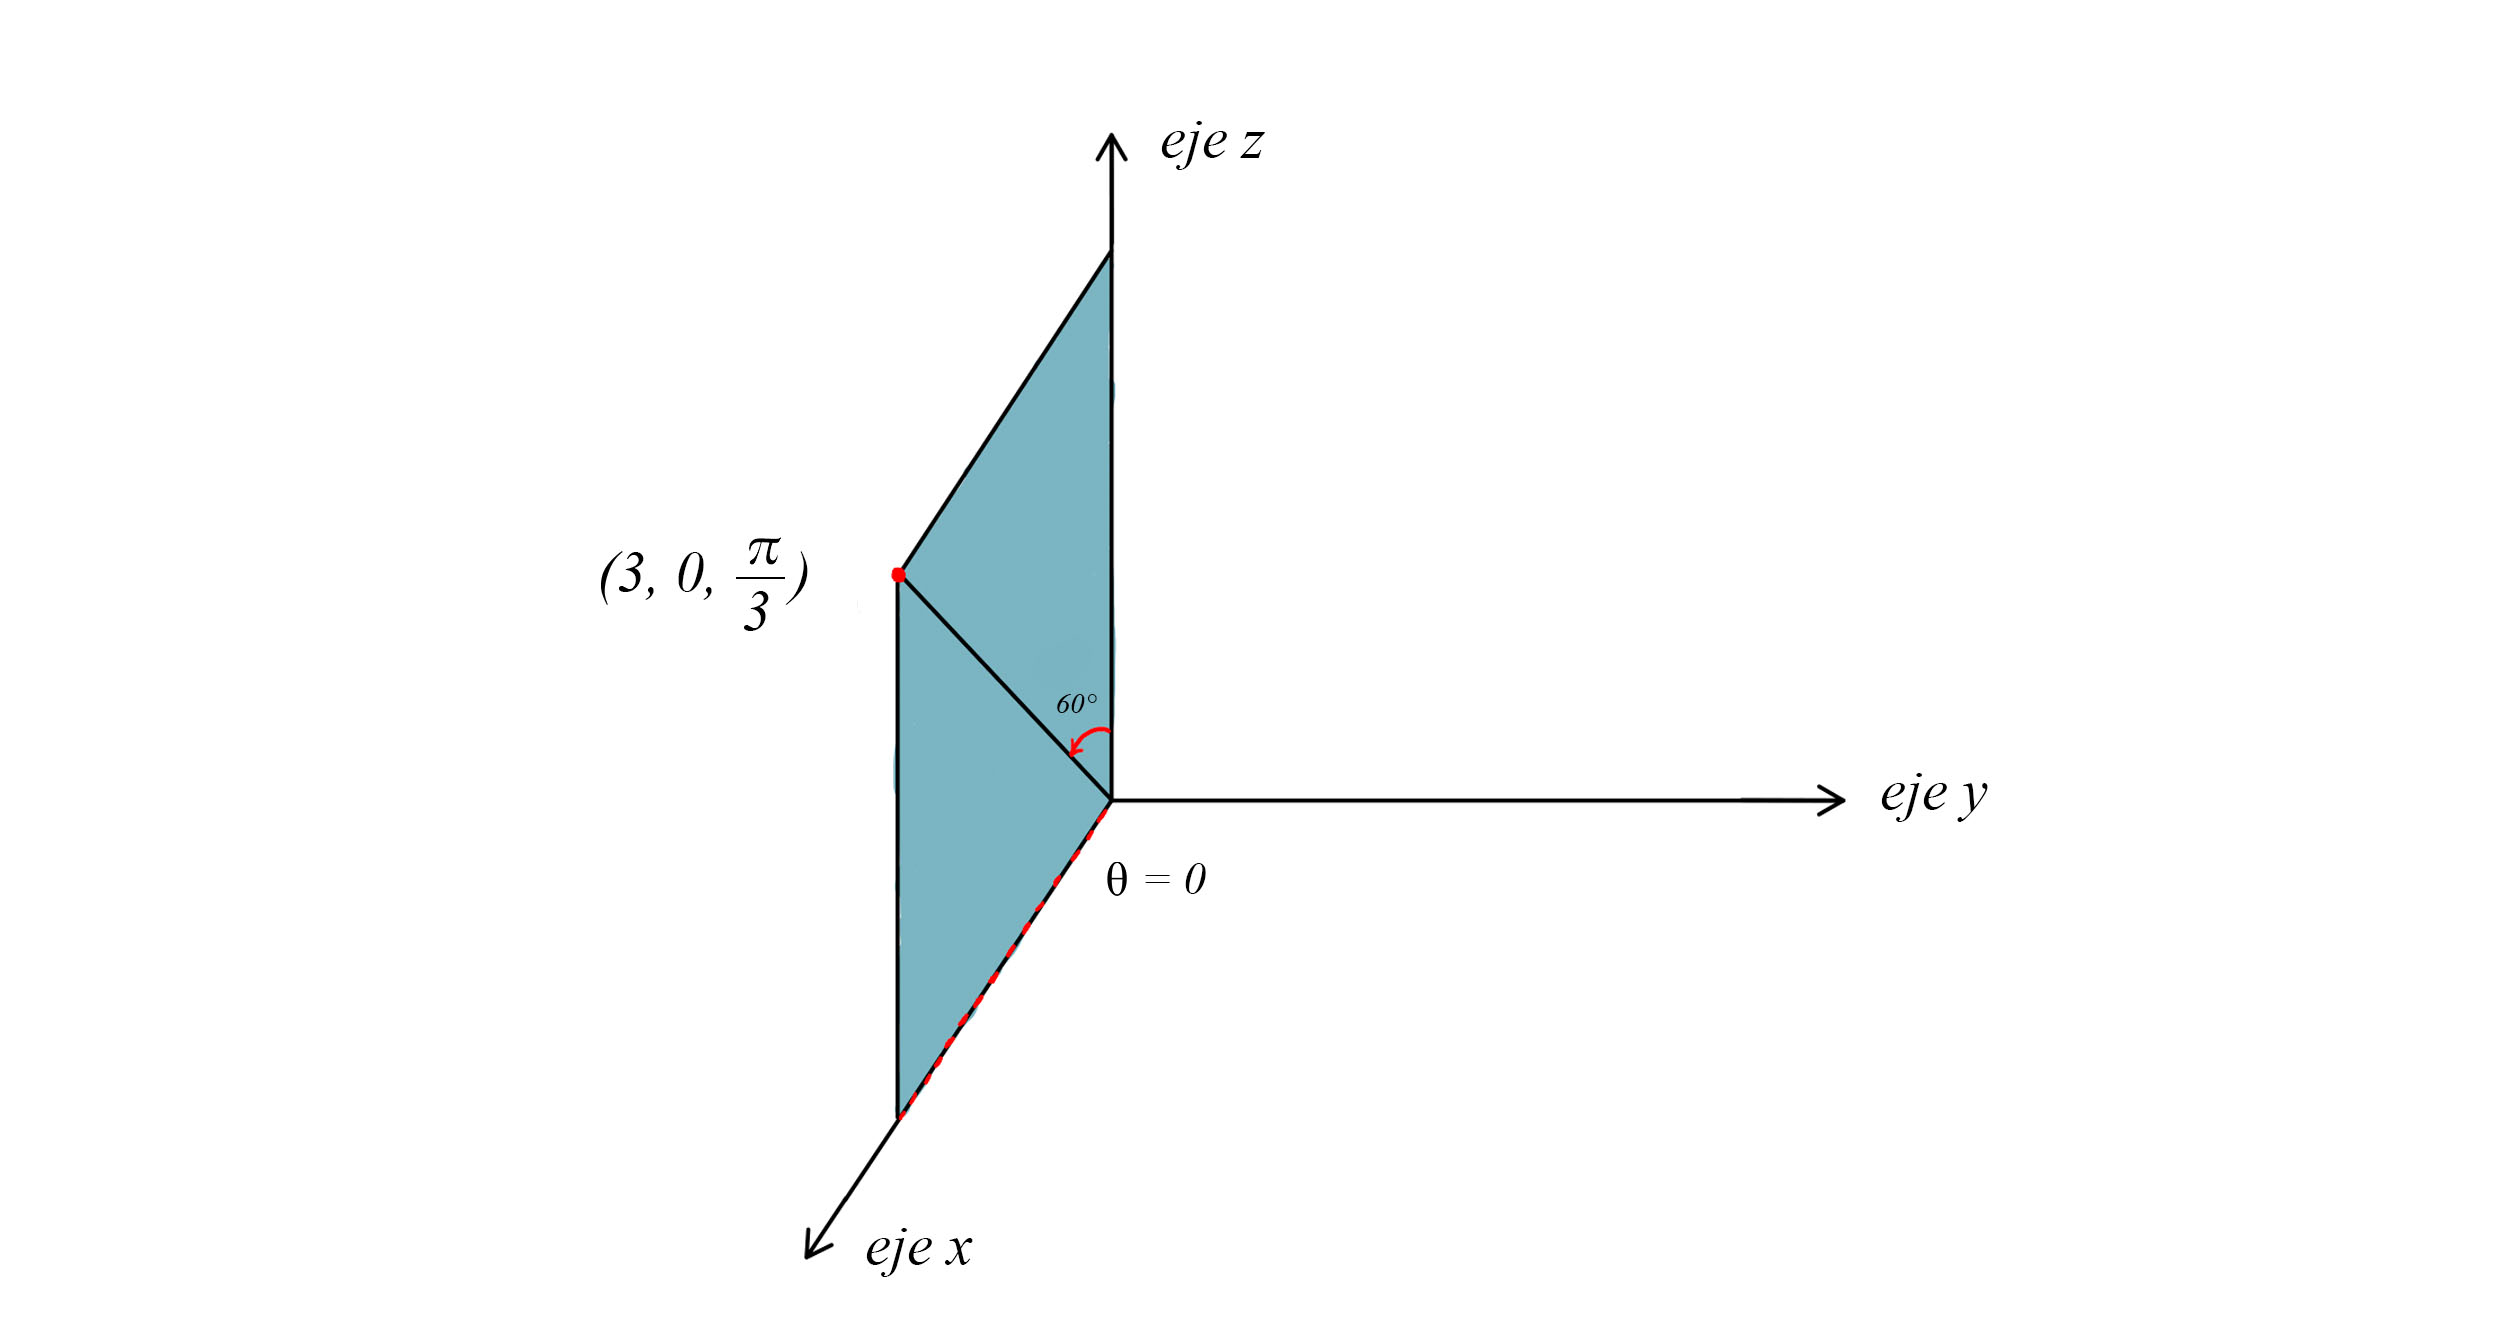
\includegraphics[width=11.17cm, height=5.97cm]{img/graph/grafica_2.jpg}
  \caption{Coordenada ${\left( 3, 0,\frac{\pi}{3} \right)}$.}
\end{figure}

\vspace{4mm}
Gráfica de la coordenada ${\left( 4, -\pi,\frac{\pi}{3} \right)}$, donde: ${\theta = -\pi = -180^{\circ} \text{ y } \varphi = \frac{\pi}{3} = 60^{\circ} }$.
\begin{figure}[H]
  \centering
  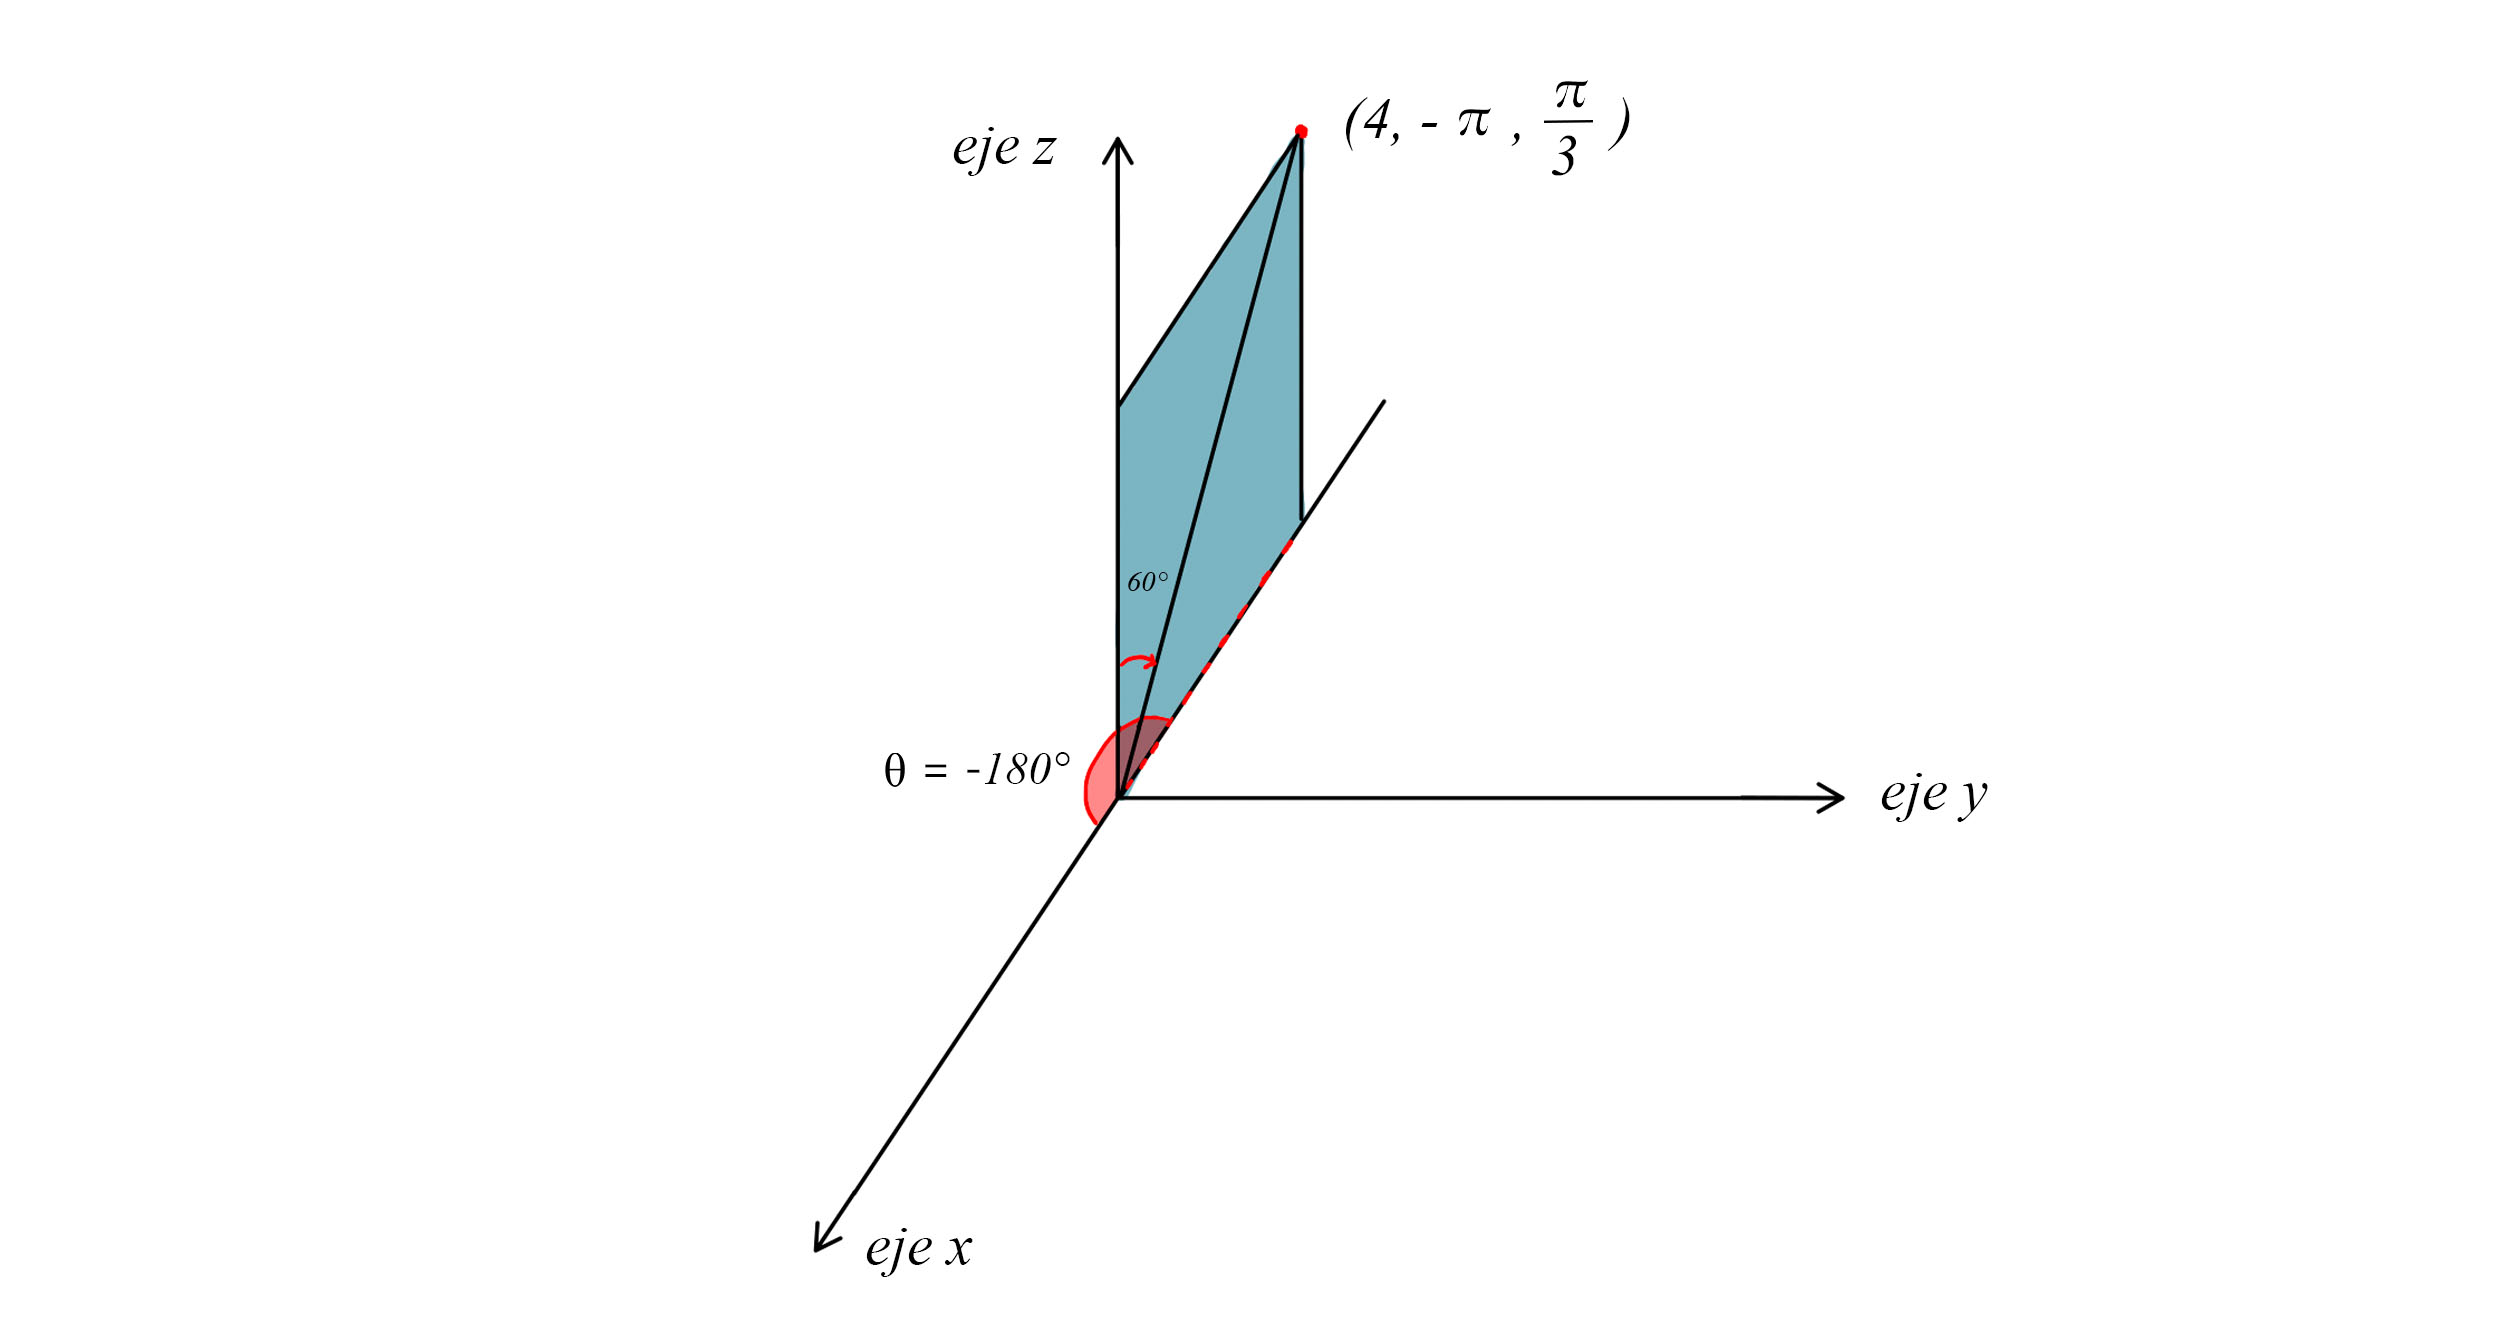
\includegraphics[width=11.17cm, height=5.97cm]{img/graph/grafica_3.jpg}
  \caption{Coordenada ${\left( 4, -\pi,\frac{\pi}{3} \right)}$.}
\end{figure}
